 
Rick proposes a new collectable figurine game to a potential investor.  He would sell less valuable Bituminous Packs for $\$8$ a pack, with a bulk discount of $\$1$ off per pack for customers who buy $10$ or more Bituminous Packs.  He would sell more valuable Anthracite Packs for $\$10$ a pack, with a bulk discount of $\$2$ off per pack for customers who buy $10$ or more Anthracite Packs.  Which of the following graphs accurately reflects the purchasing options for consumers willing to spend up to $\$160$ on figurine packs?  Presume that consumers always buy the most figurines they can for the amount of money they have committed to spend.


\ifsat
	\begin{enumerate}[label=\Alph*)]
		\item \rule{0pt}{0pt}\\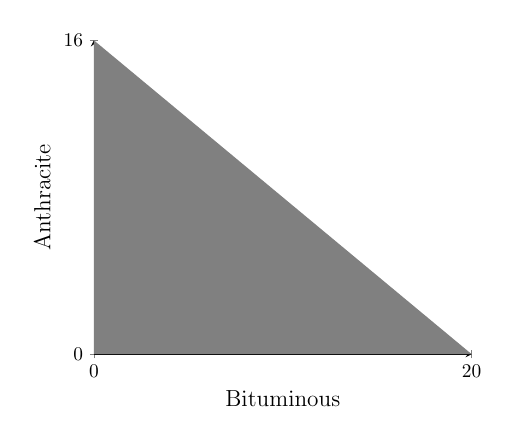
\begin{tikzpicture}[scale=0.7]\begin{axis}
 [xlabel={\large Bituminous}, ylabel={\large Anthracite}, 
 xmax=20, ymax=16, xtick={0,20}, ytick={0,16}, xmin=0, ymin=0, axis lines=left,]
 \fill[gray](axis cs:20,0)--(axis cs:0,0)--(axis cs:0,16)--cycle;
 \end{axis}\end{tikzpicture}
		\item \rule{0pt}{0pt}\\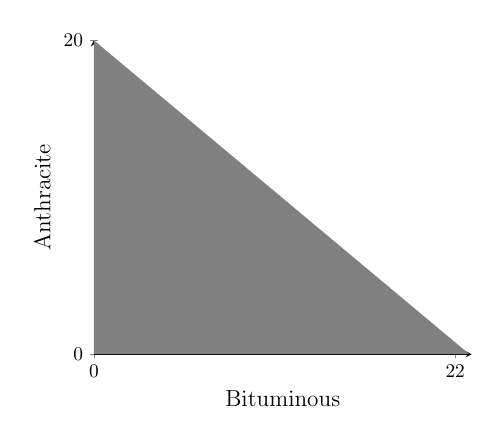
\begin{tikzpicture}[scale=0.7]\begin{axis}
 [xlabel={\large Bituminous}, ylabel={\large Anthracite}, 
 xmax=23, ymax=20, xtick={0,22}, ytick={0,20}, xmin=0, ymin=0, axis lines=left,]
 \fill[gray](axis cs:0,20)--(axis cs:0,0)--(axis cs:22.8571,0)--cycle;
 \end{axis}\end{tikzpicture}
		\item  \rule{0pt}{0pt}\\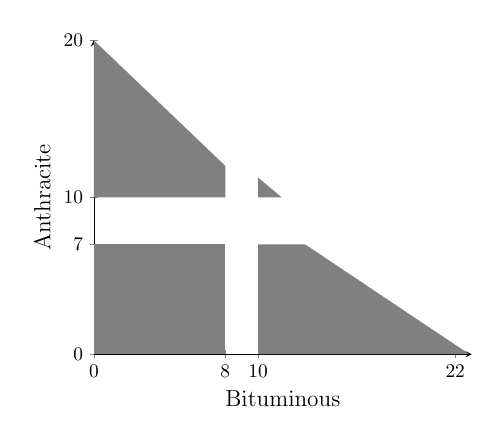
\begin{tikzpicture}[scale=0.7]\begin{axis}
 [xlabel={\large Bituminous}, ylabel={\large Anthracite}, 
 xmax=23, ymax=20, xtick={0,8,10,22}, ytick={0,7,10,20}, xmin=0, ymin=0, axis lines=left,]
 \fill[gray] (axis cs: 0,20)--(axis cs: 8,12)--(axis cs:8,10)--
 (axis cs:0,10)--cycle;
 \fill[gray] (axis cs:0,0)--(axis cs:0,7)--(axis cs:8,7)--(axis cs:8,0)
 --cycle;
 \fill[gray](axis cs:10,0)--(axis cs:10,7)--(axis cs:12.8571,7)--
 (axis cs:22.8571,0)--cycle;
 \fill[gray](axis cs:10,10)--(axis cs:10,11.25)--(axis cs:11.42857,10)
 --cycle;
 \end{axis}\end{tikzpicture} % 
		\item \rule{0pt}{0pt}\\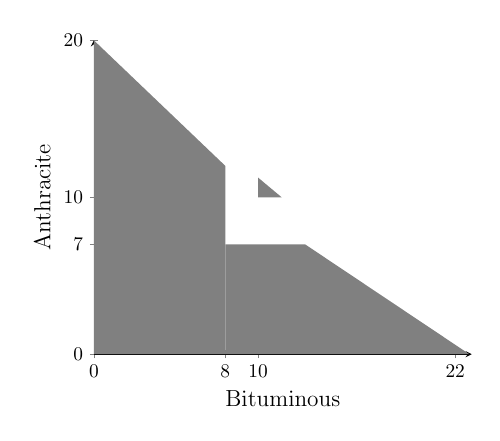
\begin{tikzpicture}[scale=0.7]\begin{axis}
 [xlabel={\large Bituminous}, ylabel={\large Anthracite}, 
 xmax=23, ymax=20, xtick={0,8,10,22}, ytick={0,7,10,20}, xmin=0, ymin=0, axis lines=left,]
 \fill[gray] (axis cs: 0,20)--(axis cs: 8,12)--(axis cs:8,0)--
 (axis cs:0,0)--cycle;
 \fill[gray](axis cs:8,0)--(axis cs:8,7)--(axis cs:12.8571,7)--
 (axis cs:22.8571,0)--cycle;
 \fill[gray](axis cs:10,10)--(axis cs:10,11.25)--(axis cs:11.42857,10)
 --cycle;
 \end{axis}\end{tikzpicture}
	\end{enumerate}
\else
\fi

\ifacteven
	\begin{enumerate}[label=\textbf{\Alph*.},itemsep=\fill,align=left]
		\setcounter{enumii}{5}
		\item  \rule{0pt}{0pt}\\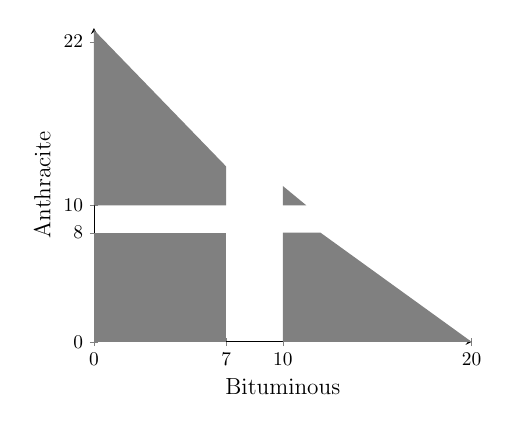
\begin{tikzpicture}[scale=0.7]\begin{axis}
 [xlabel={\large Bituminous}, ylabel={\large Anthracite}, 
 xmax=20, ymax=23, xtick={0,7,10,20}, ytick={0,8,10,22}, xmin=0, ymin=0, axis lines=left,]
 \fill[gray] (axis cs: 20,0)--(axis cs: 12,8)--(axis cs:10,8)--
 (axis cs:10,0)--cycle;
 \fill[gray] (axis cs:0,0)--(axis cs:7,0)--(axis cs:7,8)--(axis cs:0,8)
 --cycle;
 \fill[gray](axis cs:0,10)--(axis cs:7,10)--(axis cs:7,12.8571)--
 (axis cs:0,22.8571)--cycle;
 \fill[gray](axis cs:10,10)--(axis cs:11.25,10)--(axis cs:10,11.42857)
 --cycle;
 \end{axis}\end{tikzpicture}
		\item \rule{0pt}{0pt}\\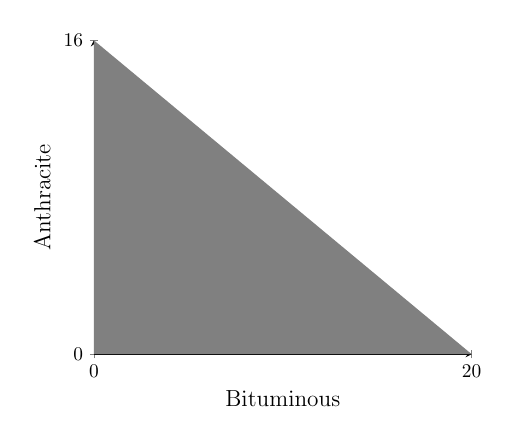
\begin{tikzpicture}[scale=0.7]\begin{axis}
 [xlabel={\large Bituminous}, ylabel={\large Anthracite}, 
 xmax=20, ymax=16, xtick={0,20}, ytick={0,16}, xmin=0, ymin=0, axis lines=left,]
 \fill[gray](axis cs:20,0)--(axis cs:0,0)--(axis cs:0,16)--cycle;
 \end{axis}\end{tikzpicture}
		\item \rule{0pt}{0pt}\\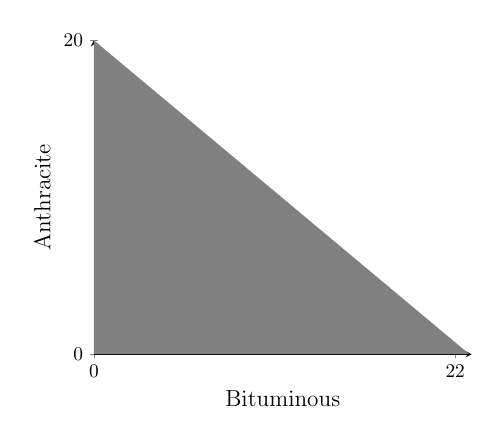
\begin{tikzpicture}[scale=0.7]\begin{axis}
 [xlabel={\large Bituminous}, ylabel={\large Anthracite}, 
 xmax=23, ymax=20, xtick={0,22}, ytick={0,20}, xmin=0, ymin=0, axis lines=left,]
 \fill[gray](axis cs:0,20)--(axis cs:0,0)--(axis cs:22.8571,0)--cycle;
 \end{axis}\end{tikzpicture}
		\addtocounter{enumii}{1}
		\item  \rule{0pt}{0pt}\\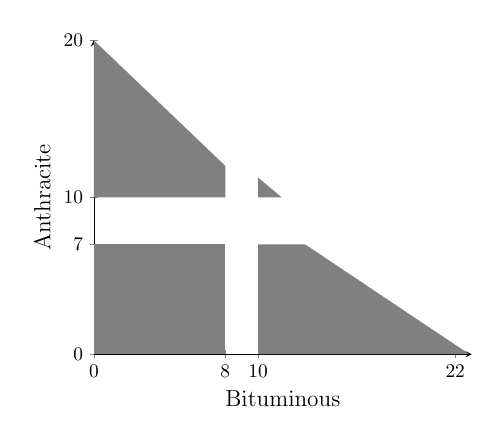
\begin{tikzpicture}[scale=0.7]\begin{axis}
 [xlabel={\large Bituminous}, ylabel={\large Anthracite}, 
 xmax=23, ymax=20, xtick={0,8,10,22}, ytick={0,7,10,20}, xmin=0, ymin=0, axis lines=left,]
 \fill[gray] (axis cs: 0,20)--(axis cs: 8,12)--(axis cs:8,10)--
 (axis cs:0,10)--cycle;
 \fill[gray] (axis cs:0,0)--(axis cs:0,7)--(axis cs:8,7)--(axis cs:8,0)
 --cycle;
 \fill[gray](axis cs:10,0)--(axis cs:10,7)--(axis cs:12.8571,7)--
 (axis cs:22.8571,0)--cycle;
 \fill[gray](axis cs:10,10)--(axis cs:10,11.25)--(axis cs:11.42857,10)
 --cycle;
 \end{axis}\end{tikzpicture} % 
		\item \rule{0pt}{0pt}\\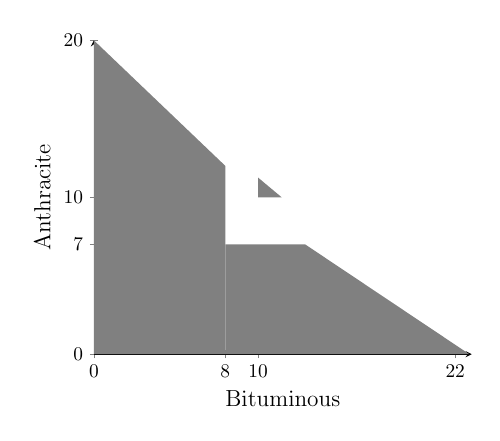
\begin{tikzpicture}[scale=0.7]\begin{axis}
 [xlabel={\large Bituminous}, ylabel={\large Anthracite}, 
 xmax=23, ymax=20, xtick={0,8,10,22}, ytick={0,7,10,20}, xmin=0, ymin=0, axis lines=left,]
 \fill[gray] (axis cs: 0,20)--(axis cs: 8,12)--(axis cs:8,0)--
 (axis cs:0,0)--cycle;
 \fill[gray](axis cs:8,0)--(axis cs:8,7)--(axis cs:12.8571,7)--
 (axis cs:22.8571,0)--cycle;
 \fill[gray](axis cs:10,10)--(axis cs:10,11.25)--(axis cs:11.42857,10)
 --cycle;
 \end{axis}\end{tikzpicture}
	\end{enumerate}
\else
\fi

\ifactodd
	\begin{enumerate}[label=\textbf{\Alph*.},itemsep=\fill,align=left]
		\item  \rule{0pt}{0pt}\\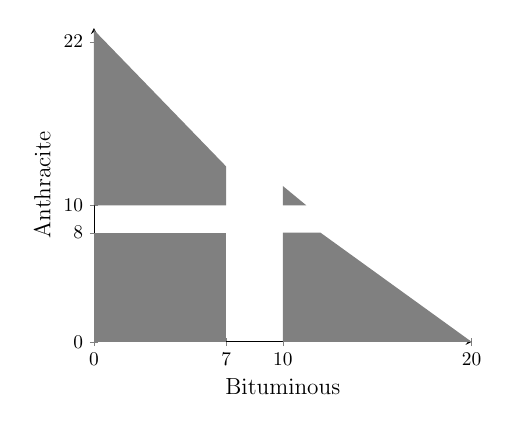
\begin{tikzpicture}[scale=0.7]\begin{axis}
 [xlabel={\large Bituminous}, ylabel={\large Anthracite}, 
 xmax=20, ymax=23, xtick={0,7,10,20}, ytick={0,8,10,22}, xmin=0, ymin=0, axis lines=left,]
 \fill[gray] (axis cs: 20,0)--(axis cs: 12,8)--(axis cs:10,8)--
 (axis cs:10,0)--cycle;
 \fill[gray] (axis cs:0,0)--(axis cs:7,0)--(axis cs:7,8)--(axis cs:0,8)
 --cycle;
 \fill[gray](axis cs:0,10)--(axis cs:7,10)--(axis cs:7,12.8571)--
 (axis cs:0,22.8571)--cycle;
 \fill[gray](axis cs:10,10)--(axis cs:11.25,10)--(axis cs:10,11.42857)
 --cycle;
 \end{axis}\end{tikzpicture}
		\item \rule{0pt}{0pt}\\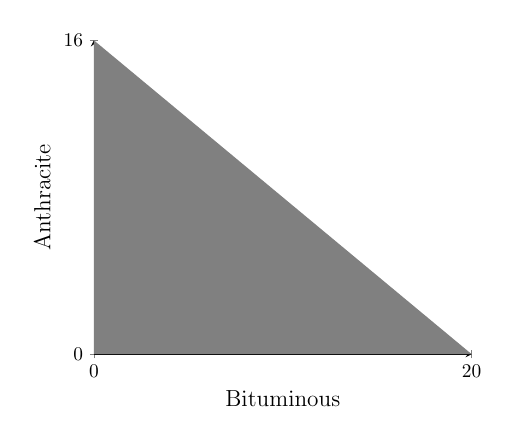
\begin{tikzpicture}[scale=0.7]\begin{axis}
 [xlabel={\large Bituminous}, ylabel={\large Anthracite}, 
 xmax=20, ymax=16, xtick={0,20}, ytick={0,16}, xmin=0, ymin=0, axis lines=left,]
 \fill[gray](axis cs:20,0)--(axis cs:0,0)--(axis cs:0,16)--cycle;
 \end{axis}\end{tikzpicture}
		\item \rule{0pt}{0pt}\\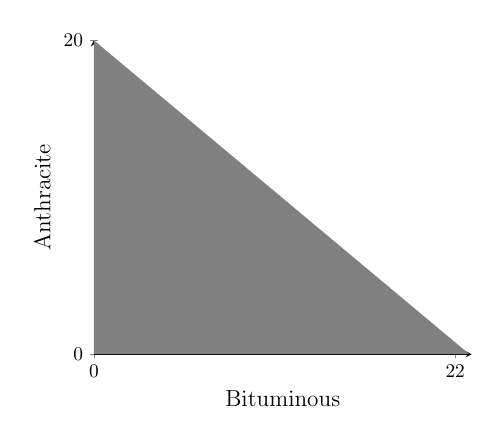
\begin{tikzpicture}[scale=0.7]\begin{axis}
 [xlabel={\large Bituminous}, ylabel={\large Anthracite}, 
 xmax=23, ymax=20, xtick={0,22}, ytick={0,20}, xmin=0, ymin=0, axis lines=left,]
 \fill[gray](axis cs:0,20)--(axis cs:0,0)--(axis cs:22.8571,0)--cycle;
 \end{axis}\end{tikzpicture}
		\item  \rule{0pt}{0pt}\\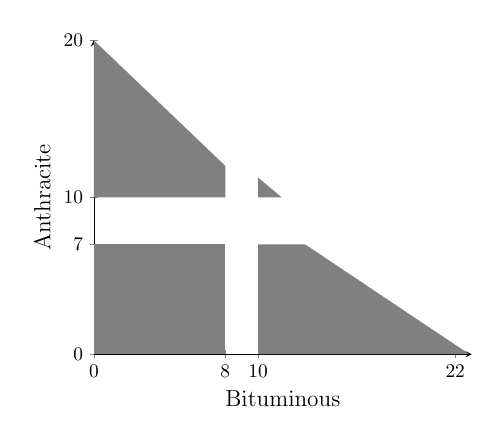
\begin{tikzpicture}[scale=0.7]\begin{axis}
 [xlabel={\large Bituminous}, ylabel={\large Anthracite}, 
 xmax=23, ymax=20, xtick={0,8,10,22}, ytick={0,7,10,20}, xmin=0, ymin=0, axis lines=left,]
 \fill[gray] (axis cs: 0,20)--(axis cs: 8,12)--(axis cs:8,10)--
 (axis cs:0,10)--cycle;
 \fill[gray] (axis cs:0,0)--(axis cs:0,7)--(axis cs:8,7)--(axis cs:8,0)
 --cycle;
 \fill[gray](axis cs:10,0)--(axis cs:10,7)--(axis cs:12.8571,7)--
 (axis cs:22.8571,0)--cycle;
 \fill[gray](axis cs:10,10)--(axis cs:10,11.25)--(axis cs:11.42857,10)
 --cycle;
 \end{axis}\end{tikzpicture} % 
		\item \rule{0pt}{0pt}\\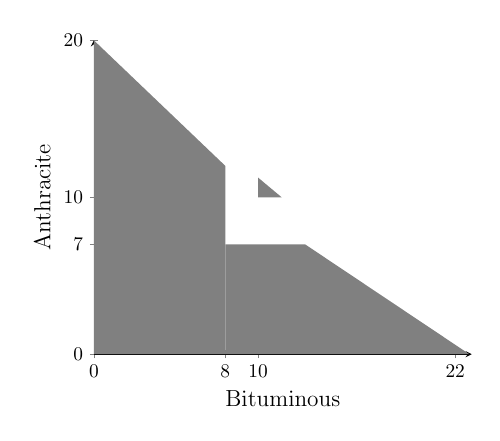
\begin{tikzpicture}[scale=0.7]\begin{axis}
 [xlabel={\large Bituminous}, ylabel={\large Anthracite}, 
 xmax=23, ymax=20, xtick={0,8,10,22}, ytick={0,7,10,20}, xmin=0, ymin=0, axis lines=left,]
 \fill[gray] (axis cs: 0,20)--(axis cs: 8,12)--(axis cs:8,0)--
 (axis cs:0,0)--cycle;
 \fill[gray](axis cs:8,0)--(axis cs:8,7)--(axis cs:12.8571,7)--
 (axis cs:22.8571,0)--cycle;
 \fill[gray](axis cs:10,10)--(axis cs:10,11.25)--(axis cs:11.42857,10)
 --cycle;
 \end{axis}\end{tikzpicture}
	\end{enumerate}
\else
\fi

\ifgridin
  \rule{0pt}{0pt}\\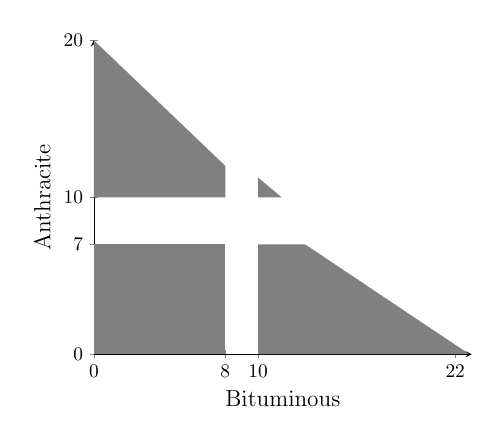
\begin{tikzpicture}[scale=0.7]\begin{axis}
 [xlabel={\large Bituminous}, ylabel={\large Anthracite}, 
 xmax=23, ymax=20, xtick={0,8,10,22}, ytick={0,7,10,20}, xmin=0, ymin=0, axis lines=left,]
 \fill[gray] (axis cs: 0,20)--(axis cs: 8,12)--(axis cs:8,10)--
 (axis cs:0,10)--cycle;
 \fill[gray] (axis cs:0,0)--(axis cs:0,7)--(axis cs:8,7)--(axis cs:8,0)
 --cycle;
 \fill[gray](axis cs:10,0)--(axis cs:10,7)--(axis cs:12.8571,7)--
 (axis cs:22.8571,0)--cycle;
 \fill[gray](axis cs:10,10)--(axis cs:10,11.25)--(axis cs:11.42857,10)
 --cycle;
 \end{axis}\end{tikzpicture} % 
		
\else
\fi

